\chapter{Results week 1}

\section{Protein concentration via BCA assay}

\label{sec:protein_concentration}

The measured absorption values at \SI{562}{\nm} of the prepared standard are
shown in table \ref{tbl:bca_absorption_standard}. Based on those, the device
calculated a linear regression:

\[
	\text{absorption} = 0.81542 \cdot \text{concentration} + 0.02701
\]

This allows calculating the concentration of the diluted samples based on their
absorption values, shown in table \ref{tbl:bca_absorption_sample}.

The measured absorption values of the standard and sample dilutions, as well as
their known respectively calculated concentrations, is further visualized in
figure \ref{fig:bca_absorption}.

Discarding the two measurements which fall outside the range of the standard,
and calculating the protein concentration of the undiluted sample, yields
concentrations of \SI{21.552}{\mg\per\ml} and \SI{17.342}{\mg\per\ml}
respectively. Using their average provides us with a protein concentration of
\SI{19.447}{\mg\per\ml}.

\begin{table}
	\centering
	\begin{tabu}{ll}
		\toprule
		Absorption & Concentration (known) \\
		\midrule
		\SI{1.6353}{OD562} & \SI{2000}{\ug\per\ml} \\
		\SI{1.2418}{OD562} & \SI{1500}{\ug\per\ml} \\
		\SI{0.8755}{OD562} & \SI{1000}{\ug\per\ml} \\
		\SI{0.6433}{OD562} & \SI{750}{\ug\per\ml} \\
		\SI{0.4756}{OD562} & \SI{500}{\ug\per\ml} \\
		\SI{0.2413}{OD562} & \SI{250}{\ug\per\ml} \\
		\SI{0.1173}{OD562} & \SI{125}{\ug\per\ml} \\
		\SI0.0225{}{OD562} & \SI{25}{\ug\per\ml} \\
		\SI{0.0053}{OD562} & \SI{0}{\ug\per\ml} \\
		\bottomrule
	\end{tabu}
	\caption{OD562 values of standard}
	\label{tbl:bca_absorption_standard}
\end{table}

\begin{table}
	\centering
	\begin{tabu}{lll}
		\toprule
		Absorption & Concentration (calculated) & Dilution factor \\
		\midrule
		\SI{2.2966}{OD562} & \SI{2783}{\ug\per\ml} & 1:5 \\
		\SI{1.8855}{OD562} & \SI{2279}{\ug\per\ml} & 1:10 \\
		\SI{0.8671}{OD562} & \SI{1030}{\ug\per\ml} & 1:20 \\
		\SI{0.5388}{OD562} & \SI{628}{\ug\per\ml} & 1:40 \\
		\bottomrule
	\end{tabu}
	\caption{OD562 values of sample dilutions}
	\label{tbl:bca_absorption_sample}
\end{table}

\begin{figure}
	\centering
	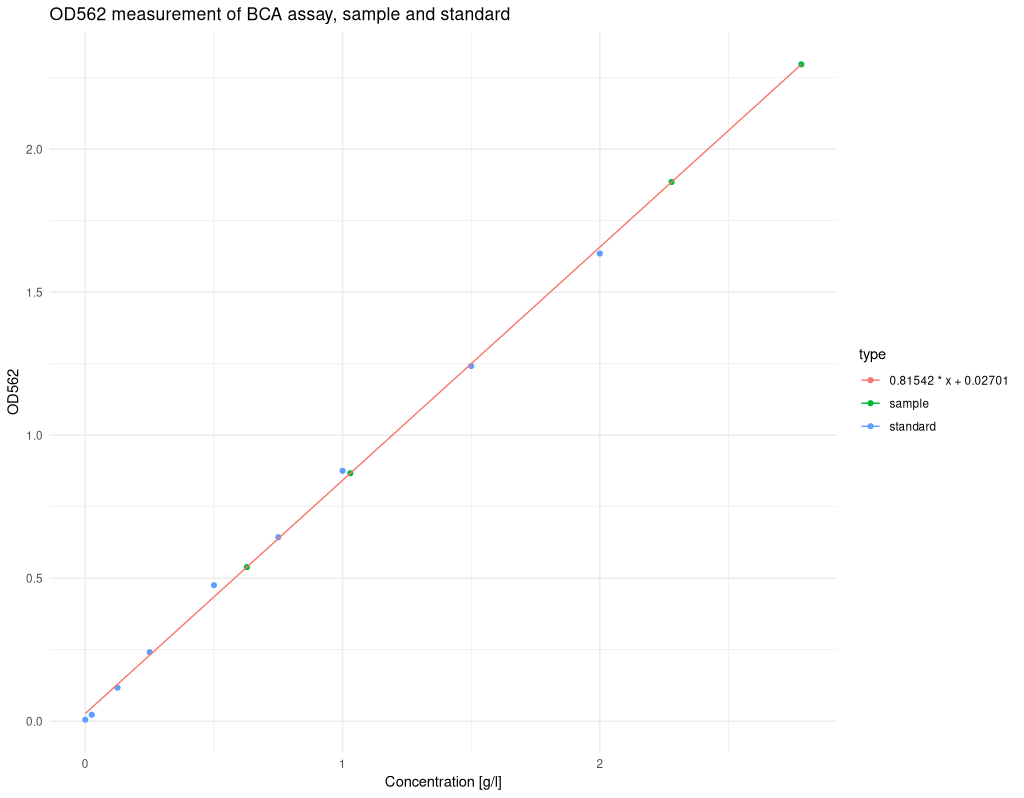
\includegraphics[width=\linewidth]{img/bca_assay.png}
	\caption{OD562 values and concentrations of standard and sample}
	\label{fig:bca_absorption}
\end{figure}

\section{Expression screening}

\subsection{OD measurements during bacterial growth}

To measure the stages of bacterial growth before and after induction, the
absorption at \SI{600}{\nm} was measured in regular intervals. These results are
found in table \ref{tbl:absorption_expression}.

As mentioned in the protocol the measurement at \SI{90}{\min} was faulty, and
was thus excluded from the visualization in figure
\ref{fig:absorption_expression}.

\begin{table}
	\centering
	\begin{tabu}{lllllllll}
		\toprule
		Medium & Rha & IPTG & \SI{0}{\min} & \SI{60}{\min} & \SI{90}{\min} & \SI{120}{\min} & \SI{200}{\min} & \SI{290}{\min} \\
		\midrule
		\csvreader[]{data/expression_od600.csv}%
		{medium=\medium,rha=\rha,iptg=\iptg,4=\tone,5=\ttwo,6=\tthree,7=\tfour,8=\tfive,9=\tsix}%
		{\\ \medium & \rha & \iptg & \tone & \ttwo& \tthree & \tfour & \tfive & \tsix}%
		\\
		\bottomrule
	\end{tabu}
	\caption{OD600 values of transformed bacteria samples}
	\label{tbl:absorption_expression}
\end{table}

\begin{figure}
	\centering
	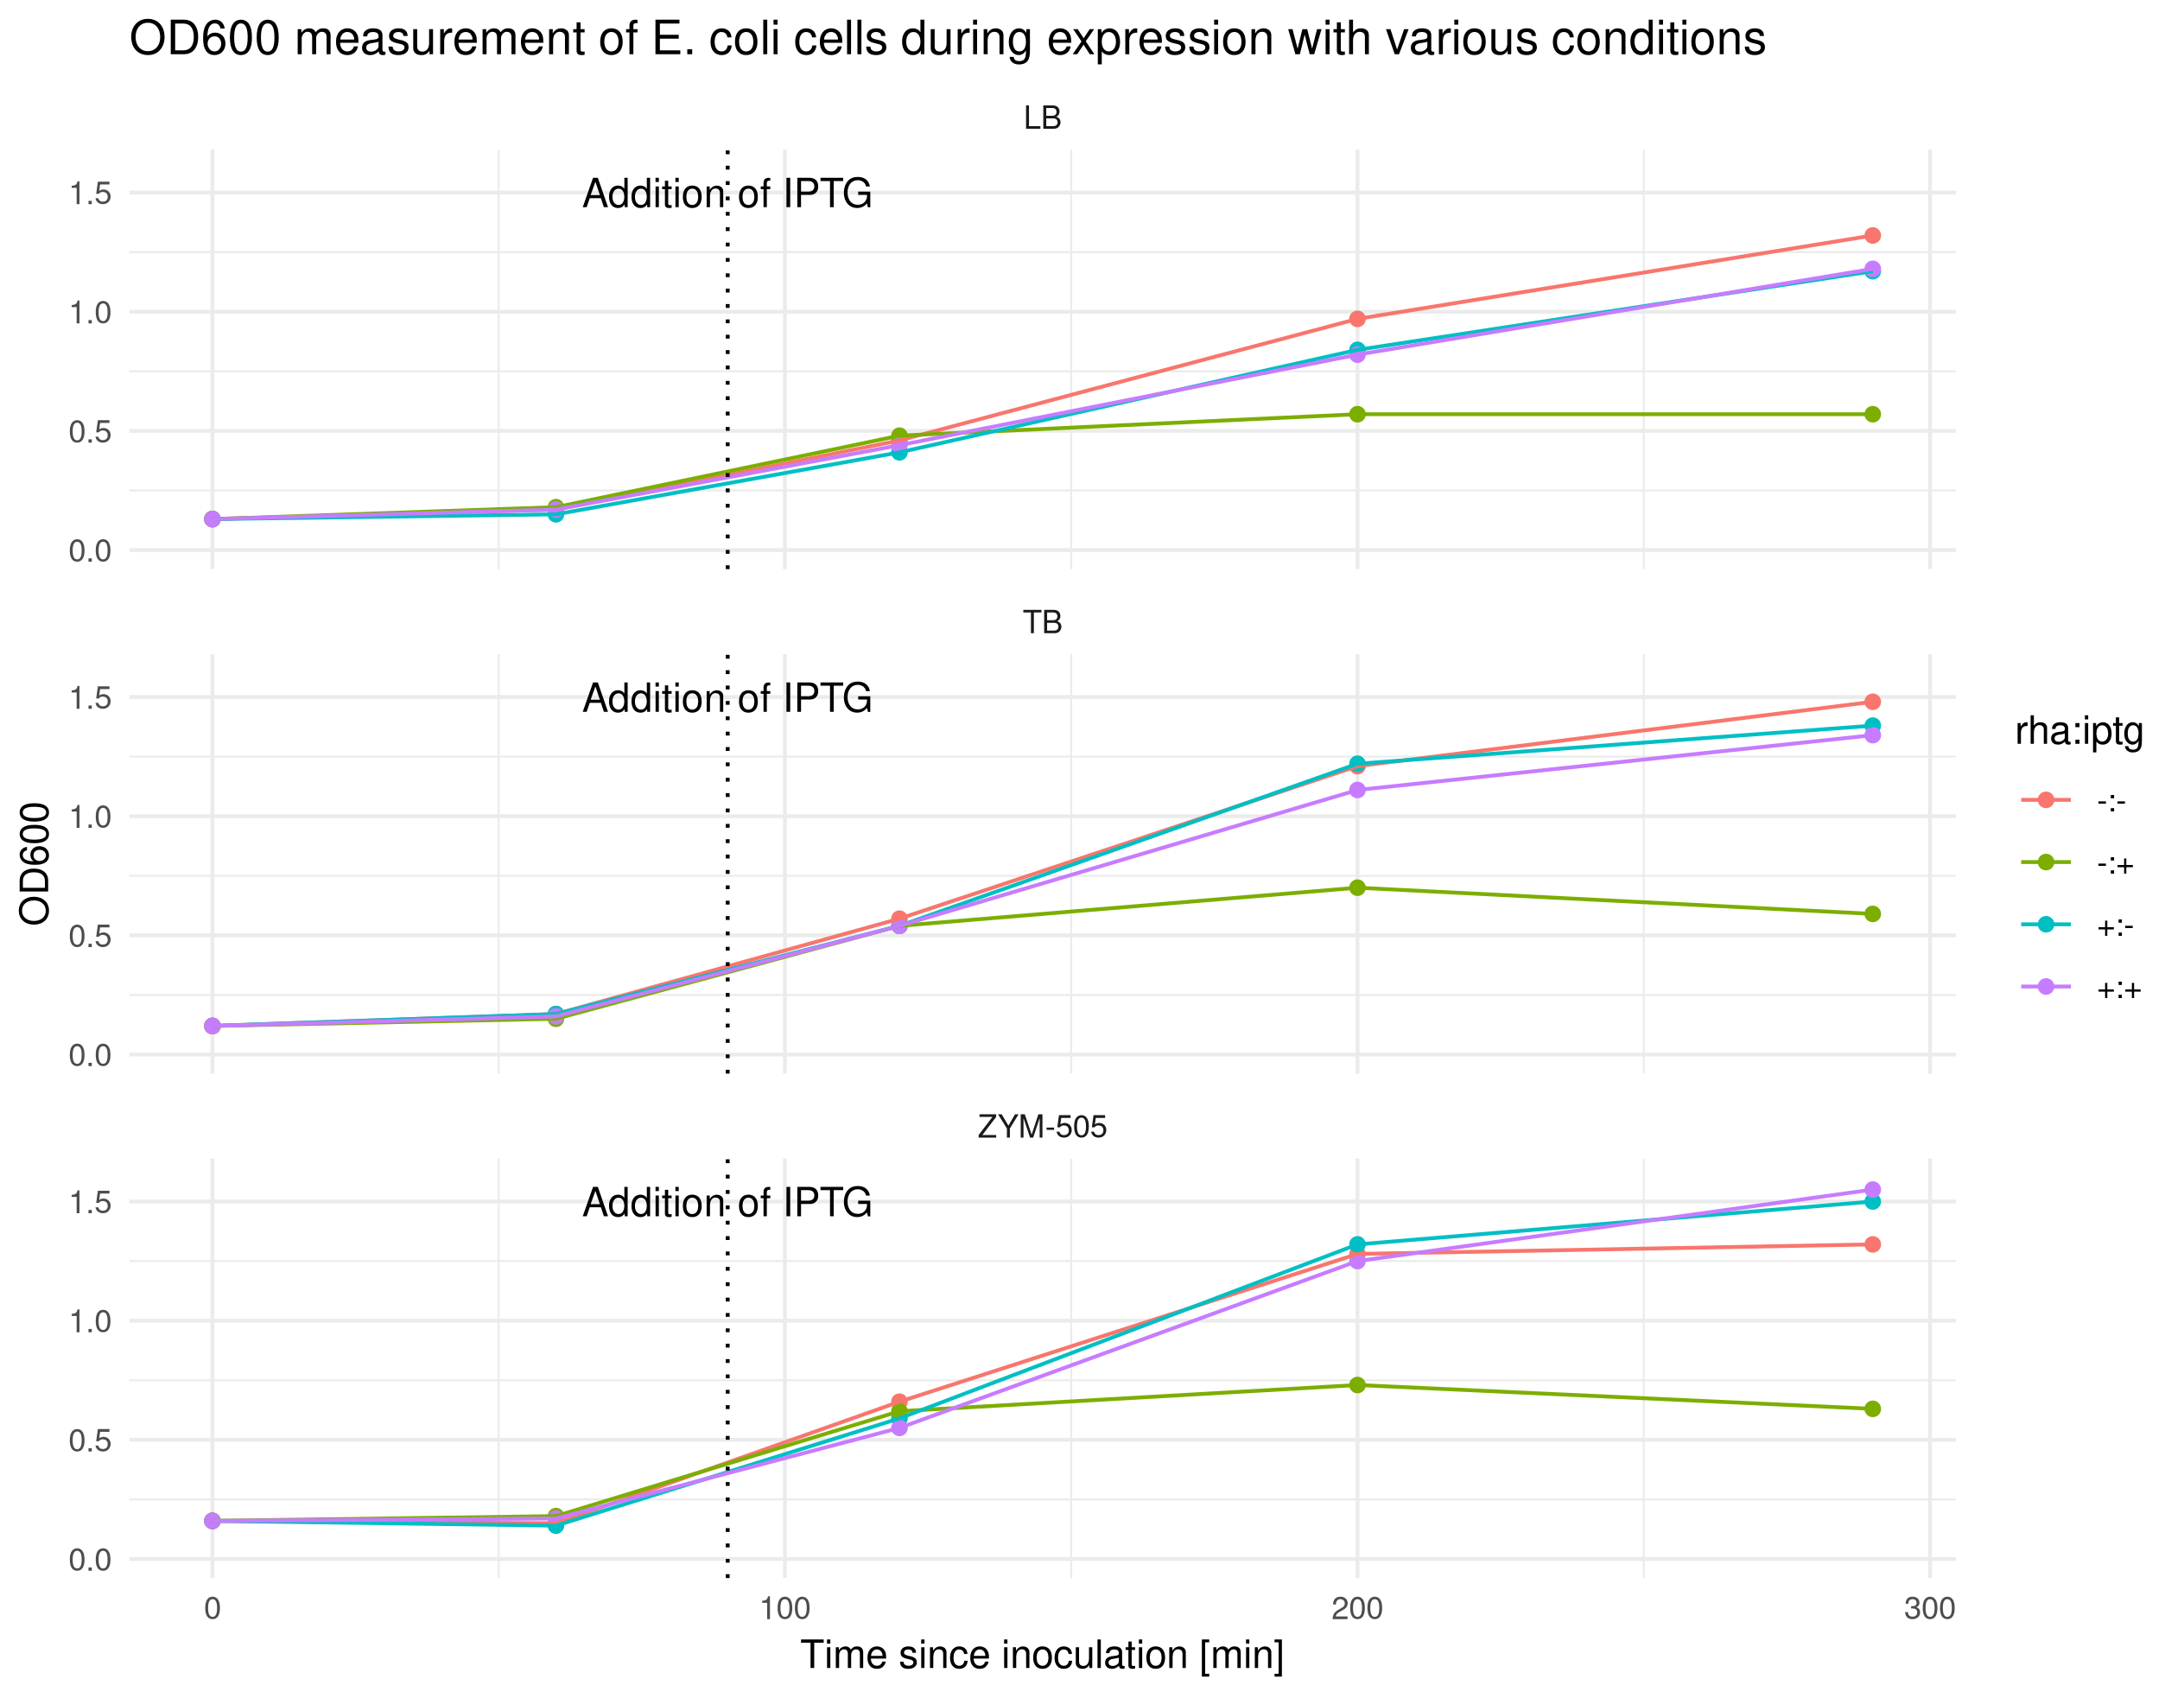
\includegraphics[width=\linewidth]{img/absorption_expression.png}
	\caption{OD600 values over time of expression samples}
	\label{fig:absorption_expression}
\end{figure}

\subsection{Fluorescence measurement}

The fluorescence measurements of the dsRed-marked protein are shown in table
\ref{tbl:expression_fluorescence}. In addition to the measured value this table
also includes the fluorescence normalized to an OD of 1, using the most recent
OD measurements. These values are further visualized in figure
\ref{fig:expression_fluorescence}.

\begin{table}
	\centering
	\begin{tabu}{llllll}
		\toprule
		Medium & Rha & IPTG & Fluorescence & Last OD$_{600}$ & Normalized fluorescence \\
		\midrule
		\csvreader[]{data/expression_fluorescence.csv}%
		{Medium=\medium,Rhamnose=\rha,IPTG=\iptg,Fluorescence=\fluorescence,5=\od,6=\fluorescencenorm}%
		{\\ \medium & \rha & \iptg & \fluorescence & \od & \fluorescencenorm}%
		\\
		\bottomrule
	\end{tabu}
	\caption{Fluorescence values of transformed bacteria samples}
	\label{tbl:expression_fluorescence}
\end{table}

\begin{figure}
	\centering
	\includegraphics[width=\linewidth]{img/expression_fluorescence.png}
	\caption{Fluorescence values of transformed bacteria samples}
	\label{fig:expression_fluorescence}
\end{figure}
